\chapter{绪论}

\section{研究背景与意义}

智慧城市与智能交通发展背景下行人导航与控制系统在现代交通管理中作用重要。行人作为城市交通系统的重要组成部分其行为具有显著随机性和多样性给传统交通管理和路径规划方法带来诸多挑战,行人导航系统研究旨在通过实时路径优化与智能调控提升行人交通安全与出行效率。但传统导航方法多基于规则模型主要依赖静态预设参数,难以应对复杂动态环境中行人行为的快速变化,比如面对突发障碍物或密集交通流动时传统算法常无法快速调整路径规划或实时优化决策进而影响导航系统可靠性与安全性。

近年来人工智能技术快速发展,强化学习作为数据驱动的决策优化方法为行人导航领域提供全新思路,其通过智能体与环境交互学习最优策略能在动态环境中实现实时决策优化,特别适用于非线性非结构化的复杂场景。不过仅依靠强化学习技术难以全面解决行人导航问题,现实环境中数据采集的高成本高风险特性在实际应用中极大限制了强化学习的训练与推广。

\begin{figure}[H]
    \centering
    \begin{subfigure}{0.48\textwidth}
        
\includegraphics[width=\linewidth]{images/Unreal_Engine.pdf}
    \end{subfigure}
    \hfill 
    \begin{subfigure}{0.48\textwidth}
        
\includegraphics[width=\linewidth]{images/Carla.pdf}
    \end{subfigure}
    \caption{虚幻引擎和Carla}
    \label{fig:CarlaUE}
\end{figure}

本研究基于 Carla 利用虚幻引擎(Unreal Engine)这一高仿真度虚拟场景构建平台提供了解决实际环境数据采集困难的理想工具,如图 \ref{fig:CarlaUE}所示。该引擎既能生成复杂多样的动态环境也能模拟真实场景中行人行为的随机性和多样性,为强化学习智能体的训练与测试提供安全低成本的实验平台。如通过虚幻引擎模拟十字路口复杂交通场景可逼真再现行人与车辆的动态交互,为强化学习算法的优化与验证创造实验条件,且其支持生成视觉、惯性、语义信息等多种传感器数据进一步丰富了强化学习的训练数据来源。

本研究结合虚拟仿真技术和强化学习算法解决行人导航核心问题,包括精准建模动态环境下行人行为,行人行为受交通信号、周围车辆动态变化及其他行人行为等多种因素影响,建立能真实反映不同环境中行人决策逻辑的高精度行人行为模型是首要难题;高效结合虚拟仿真与强化学习,强化学习有效性依赖训练环境质量,虚幻引擎仿真能力为训练高效智能体提供可能,但设计能充分利用虚幻引擎生成的多样化数据的高效强化学习算法亟待解决;平衡路径规划效率与行人安全性,行人导航系统要提高路径规划效率并优先考虑行人安全,如在交通高峰期复杂场景中找到安全高效路径是研究重点。

智慧交通系统发展对行人导航系统提出更高要求,既需与车辆、交通信号灯等其他交通参与者无缝协作以优化交通系统运行效率,随着多智能体技术发展,行人导航系统研究也从单一智能体优化转向多智能体协作,通过多智能体协同作用提升导航效率与安全性是未来重要研究方向。

本研究引入虚幻引擎仿真能力与强化学习自适应策略优化能力试图突破上述问题,虚幻引擎的逼真场景和多样化数据为复杂行为建模和智能体训练提供支持,强化学习算法自适应优化能力使智能体可快速适应复杂动态环境变化,两者结合能为行人导航系统提供新理论和技术支撑,在智能交通、自动驾驶和城市规划等领域有广泛应用潜力。

\section{国内外研究现状}

近年来强化学习与虚拟仿真技术在智能交通和行人导航领域研究取得显著进展,从强化学习在行人导航中的应用、虚幻引擎在智能体训练中的作用以及行人导航的挑战与发展趋势三方面进行综述。

\subsection{强化学习在行人导航中的应用}

强化学习(Reinforcement Learning, RL)是一种通过智能体与环境交互学习最优策略的方法,近年来在交通系统优化和行人导航中得到了广泛应用。与传统路径规划方法相比,强化学习不仅可以应对动态环境,还能通过不断训练提高系统性能,展现了较高的自适应性和优化能力。强化学习技术在交通信号控制取得重要成果,钱立军等\cite{qian2024sac}基于 SAC 算法优化多交叉口交通信号控制提升交通通行效率,为动态环境复杂信号调度提供新思路,Arulkumaran等\cite{arulkumaran2017deeprl}系统阐述了深度强化学习在动态决策中的理论优势,Wei 等\cite{wei2021survey}综述强化学习在交通信号控制研究进展指出深度强化学习(Deep Reinforcement Learning, DRL)解决非线性优化问题优势适用于实时动态交通场景;在路径规划领域应用广泛,陶幸等\cite{tao2024motion}提出基于惯性传感器免对准动作捕捉方法为动态场景行人行为建模提供技术支持,Chen 等\cite{chen2018ionet}结合深度学习与强化学习技术设计基于因果推理路径优化方法引入因果关系提升智能体在动态环境适应能力;深度强化学习为路径规划研究注入新动力,Mnih 等\cite{mnih2013dqn}首次提出深度 Q 学习(Deep Q - Learning, DQN)算法将深度神经网络引入强化学习框架提升其在高维状态空间表现能力;在多智能体协作问题广泛研究,Clifton等\cite{clifton2020qlearning}系统论证了Q-learning算法在动态决策中的理论优势,Lian 等\cite{lian2023inverseql}设计基于离线 Q 学习多智能体协作算法解决复杂动态场景全局优化问题,Zhang等\cite{zhang2019pedestrian}提出的行人安全感知信号控制策略,Yazdani等\cite{yazdani2023ivpl}开发的IVPL系统进一步验证了深度强化学习在行人优先信号控制中的有效性,厦门路桥信息\cite{xiamen2025}开发的碰撞预测系统通过多智能体实时交互,将高风险路口预警准确率提升至89\%。Luo等\cite{luo2023adaptive}提出的自适应道路配置算法通过分布式强化学习范式,在行人流量动态调整中实现了49.55\%的计算成本优化。

\subsection{虚幻引擎在智能体训练中的作用}

虚幻引擎作为高仿真虚拟场景构建工具为复杂动态环境下强化学习算法训练和验证提供高效实验平台,借由强大虚拟仿真能力和多样化场景支持成为智能体训练测试重要工具。

1. \textbf{虚幻引擎在视觉导航研究中的应用:} 虚幻引擎在视觉导航研究应用广泛,Redmon等\cite{redmon2017yolo9000}通过虚幻引擎生成增强数据训练 YOLO 目标检测模型,Mourikis 等\cite{mourikis2007msckf}结合虚幻引擎构建视觉惯性导航系统并通过多状态约束卡尔曼滤波(MSCKF)算法优化路径规划,Howard等\cite{howard2017mobilenets}提出的轻量化网络为实时目标检测提供了重要技术支持,Campos 等\cite{campos2021orbslam3}提出的 ORB-SLAM3 算法利用虚拟场景数据显著提升视觉建图与定位的鲁棒性和精度为复杂动态环境中的导航提供有力支持,DSR-YOLO模型\cite{dsryolo2025}通过集成DCNv4和SimAM注意力机制,在CityPersons数据集上实现70.25\%的mAP@50。STI-Bench基准测试\cite{sti2025}显示当前多模态大模型在时空量化任务中平均准确率不足42\%。

2. \textbf{虚幻引擎在路径规划中的贡献:} 虚幻引擎于路径规划研究表现重要作用,Guo 等\cite{guo2020pdr}结合虚幻引擎动态仿真能力提出基于 PDR/UWB 融合的导航系统用于复杂环境行人路径优化,Wang 等\cite{wang2023llio}通过虚幻引擎构建高仿真交通场景训练强化学习智能体路径规划策略验证其在强化学习训练中的高效性和低成本特性。

3. \textbf{虚幻引擎与目标检测的结合:} 虚幻引擎还被用于目标检测与路径规划结合研究,Redmon 等\cite{redmon2017yolo9000}通过虚幻引擎生成增强数据训练 YOLO 目标检测模型提高目标检测在复杂场景中的表现能力,Ren等\cite{ren2017fasterrcnn}提出的目标检测框架为动态障碍物识别提供了新思路,Zhang等\cite{zhang2023shapeiou}提出的Shape-IoU指标为动态障碍物检测精度评估提供了更优的度量标准,Simonyan 和 Zisserman 等\cite{simonyan2014action}进一步研究虚幻引擎对深度学习模型的优化作用为复杂交通场景下的行为预测提供理论支持。 

4. \textbf{虚幻引擎在多智能体协作中的应用:} 虚幻引擎的仿真能力在多智能体协作研究中广泛应用,Bochkovskiy 等\cite{bochkovskiy2020yolov4}开发基于虚幻引擎的交通流量仿真工具验证多智能体协作算法有效性,Campos 等\cite{campos2021orbslam3}通过虚拟场景数据验证智能体在多智能体协作场景中的优化表现为行人导航系统的多智能体研究提供重要支持,Liu等\cite{liu2020tlio}通过紧耦合学习方法改进了惯性里程计精度。

虚幻引擎为强化学习算法设计训练与验证提供有力支持,在视觉导航路径规划与多智能体协作中的应用展现巨大潜力。

\subsection{行人导航的挑战与发展趋势}

行人导航技术虽取得显著进展但在复杂动态环境中仍存复杂行为建模、动态环境适应性及多智能体协作优化等诸多挑战。

1. \textbf{行人行为的复杂建模:} 行人行为具显著多样性与随机性,赵靖等\cite{zhao2014crossing}提出基于动态信号优化的行人过街模型通过行为建模提升信号控制效率与安全性,Foxlin 等\cite{foxlin2005tracking}设计基于惯性传感器的行人轨迹跟踪方法为复杂行为建模提供技术支持。长沙智慧信号灯系统\cite{changsha2021}通过LED动态提示和900万像素违法抓拍单元显著减少路口事故,Zhang等\cite{zhang2025traffic}开发的MFS-MSTD模型在非随机缺失场景下流量修复误差降低52\%。

2. \textbf{动态环境的实时适应:} 动态环境不确定性对导航系统提出更高要求,Herath 等\cite{herath2020ronin}通过视觉信号优化路径规划使智能体实时适应动态障碍物变化,Dai等\cite{dai2017temporalcontext}提出的时序上下文网络为动态行为预测提供了新方法,Wang 等\cite{wang2013densetrajectory}提出基于强化学习的信号优化方法在动态环境中提升系统鲁棒性,Reid等\cite{reid1980tracking}提出的多目标跟踪算法为动态障碍物预测提供了理论基础。

3. \textbf{多智能体协作的优化:} 复杂交通场景中多智能体协作优化问题尤为重要,Lian 等\cite{lian2023inverseql}通过强化学习实现多智能体高效协作提高全局路径规划效率,Campos 等\cite{campos2021orbslam3}利用虚幻引擎验证多智能体协作优化算法在复杂场景中的应用价值。叶军华\cite{ye2023fusion}提出的多传感器融合定位算法将室内定位误差降低至3米以内。

4. \textbf{未来研究趋势:} 未来行人导航研究将朝以下方向发展:基于多源数据的复杂行为建模与优化;提升强化学习智能体在动态环境中的泛化能力;多智能体协作优化在虚拟仿真环境中的深度应用。

\section{研究内容与创新}

本研究聚焦 "基于虚幻引擎的行人强化学习控制与导航系统" 展开,针对复杂动态交通环境中行人智能导航问题,运用虚拟仿真平台 Carla 与强化学习算法构建可训练、可评估、可扩展的智能导航系统。具体研究内容如下:

1. \textbf{构建高仿真虚拟行人导航环境} 基于虚幻引擎与 Carla 平台构建高仿真虚拟行人导航环境,通过模拟城市道路结构、交通信号、车辆动态、障碍物变化等因素建立支持多场景切换的训练测试环境,形成高逼真度虚拟实验平台为智能体学习提供真实感知基础。

2. \textbf{设计多行为控制与骨骼建模系统:} 设计多行为控制与骨骼建模系统,借助 Carla 平台控制 API 及骨骼动画控制机制实现行人单向行走、过马路、来回走动等基础行为建模和动态路径更新,提升系统对多样化行人行为的响应能力。

3. \textbf{引入并比较多种强化学习算法:} 引入 PID 控制、DQN 算法、PPO 算法三种强化学习控制策略,在避障成功率、路径规划效率、模型稳定性等方面对比其性能表现,通过实验评估算法在动态环境中的适应性与可推广性。

4. \textbf{构建可解释性奖励函数体系:} 结合行人实际行为及交通安全需求构建可解释性奖励函数体系,设计融合目标达成、路径跟踪、安全避障、时间效率等因素的多维奖励函数,增强模型对复杂目标的理解与优化能力。

5. \textbf{实现系统性能评估与可视化展示:} 开展系统性能评估与可视化展示工作,通过仿真实验分析不同算法控制下的导航路径、碰撞率、目标达成时间等指标,利用图像增强与日志分析技术对行人导航过程进行可视化呈现,为后续系统优化与部署提供辅助支持。

本研究创新性体现在:

1. \textbf{融合虚拟仿真与强化学习:} 融合虚拟仿真与强化学习搭建低成本高精度训练平台,借助虚幻引擎生成可控多样场景,解决传统现实数据采集难度大、风险高的问题,实现强化学习模型安全训练与快速迭代。

2. \textbf{提出动态加权融合路径规划机制:} 在 PID 控制中设计目标向量与避障向量的动态加权机制,结合雷达感知与环境反馈提升行人智能体对突发障碍的响应能力。

3. \textbf{构建多维奖励函数促进多目标导航优化:} 基于导航目标与交通安全性构建复合奖励函数体系,兼顾目标达成速度、路径偏差、避障效果与行走合理性,推动智能体学习策略从单一任务导向转向多目标协同优化。

4. \textbf{完成 DQN 与 PPO 两种主流强化学习算法在复杂交通环境中的对比分析:} 首次在 Carla 行人控制任务中系统对比两类深度强化学习方法的表现,提出适用于动态城市环境的稳定策略优化路径。

通过上述研究,该系统展示了虚拟仿真与强化学习在智慧交通中的深度融合潜力,为未来多智能体行人交通协同控制提供理论参考与实验平台支撑。

\section{论文组织架构}

本论文以 "基于虚幻引擎的行人强化学习控制与导航系统" 为主题,针对智慧城市交通场景下复杂行人导航问题展开研究,内容涵盖仿真平台构建、强化学习算法实现、导航系统设计、实验验证与未来发展等方面。

\begin{figure}[H]
    \centering
    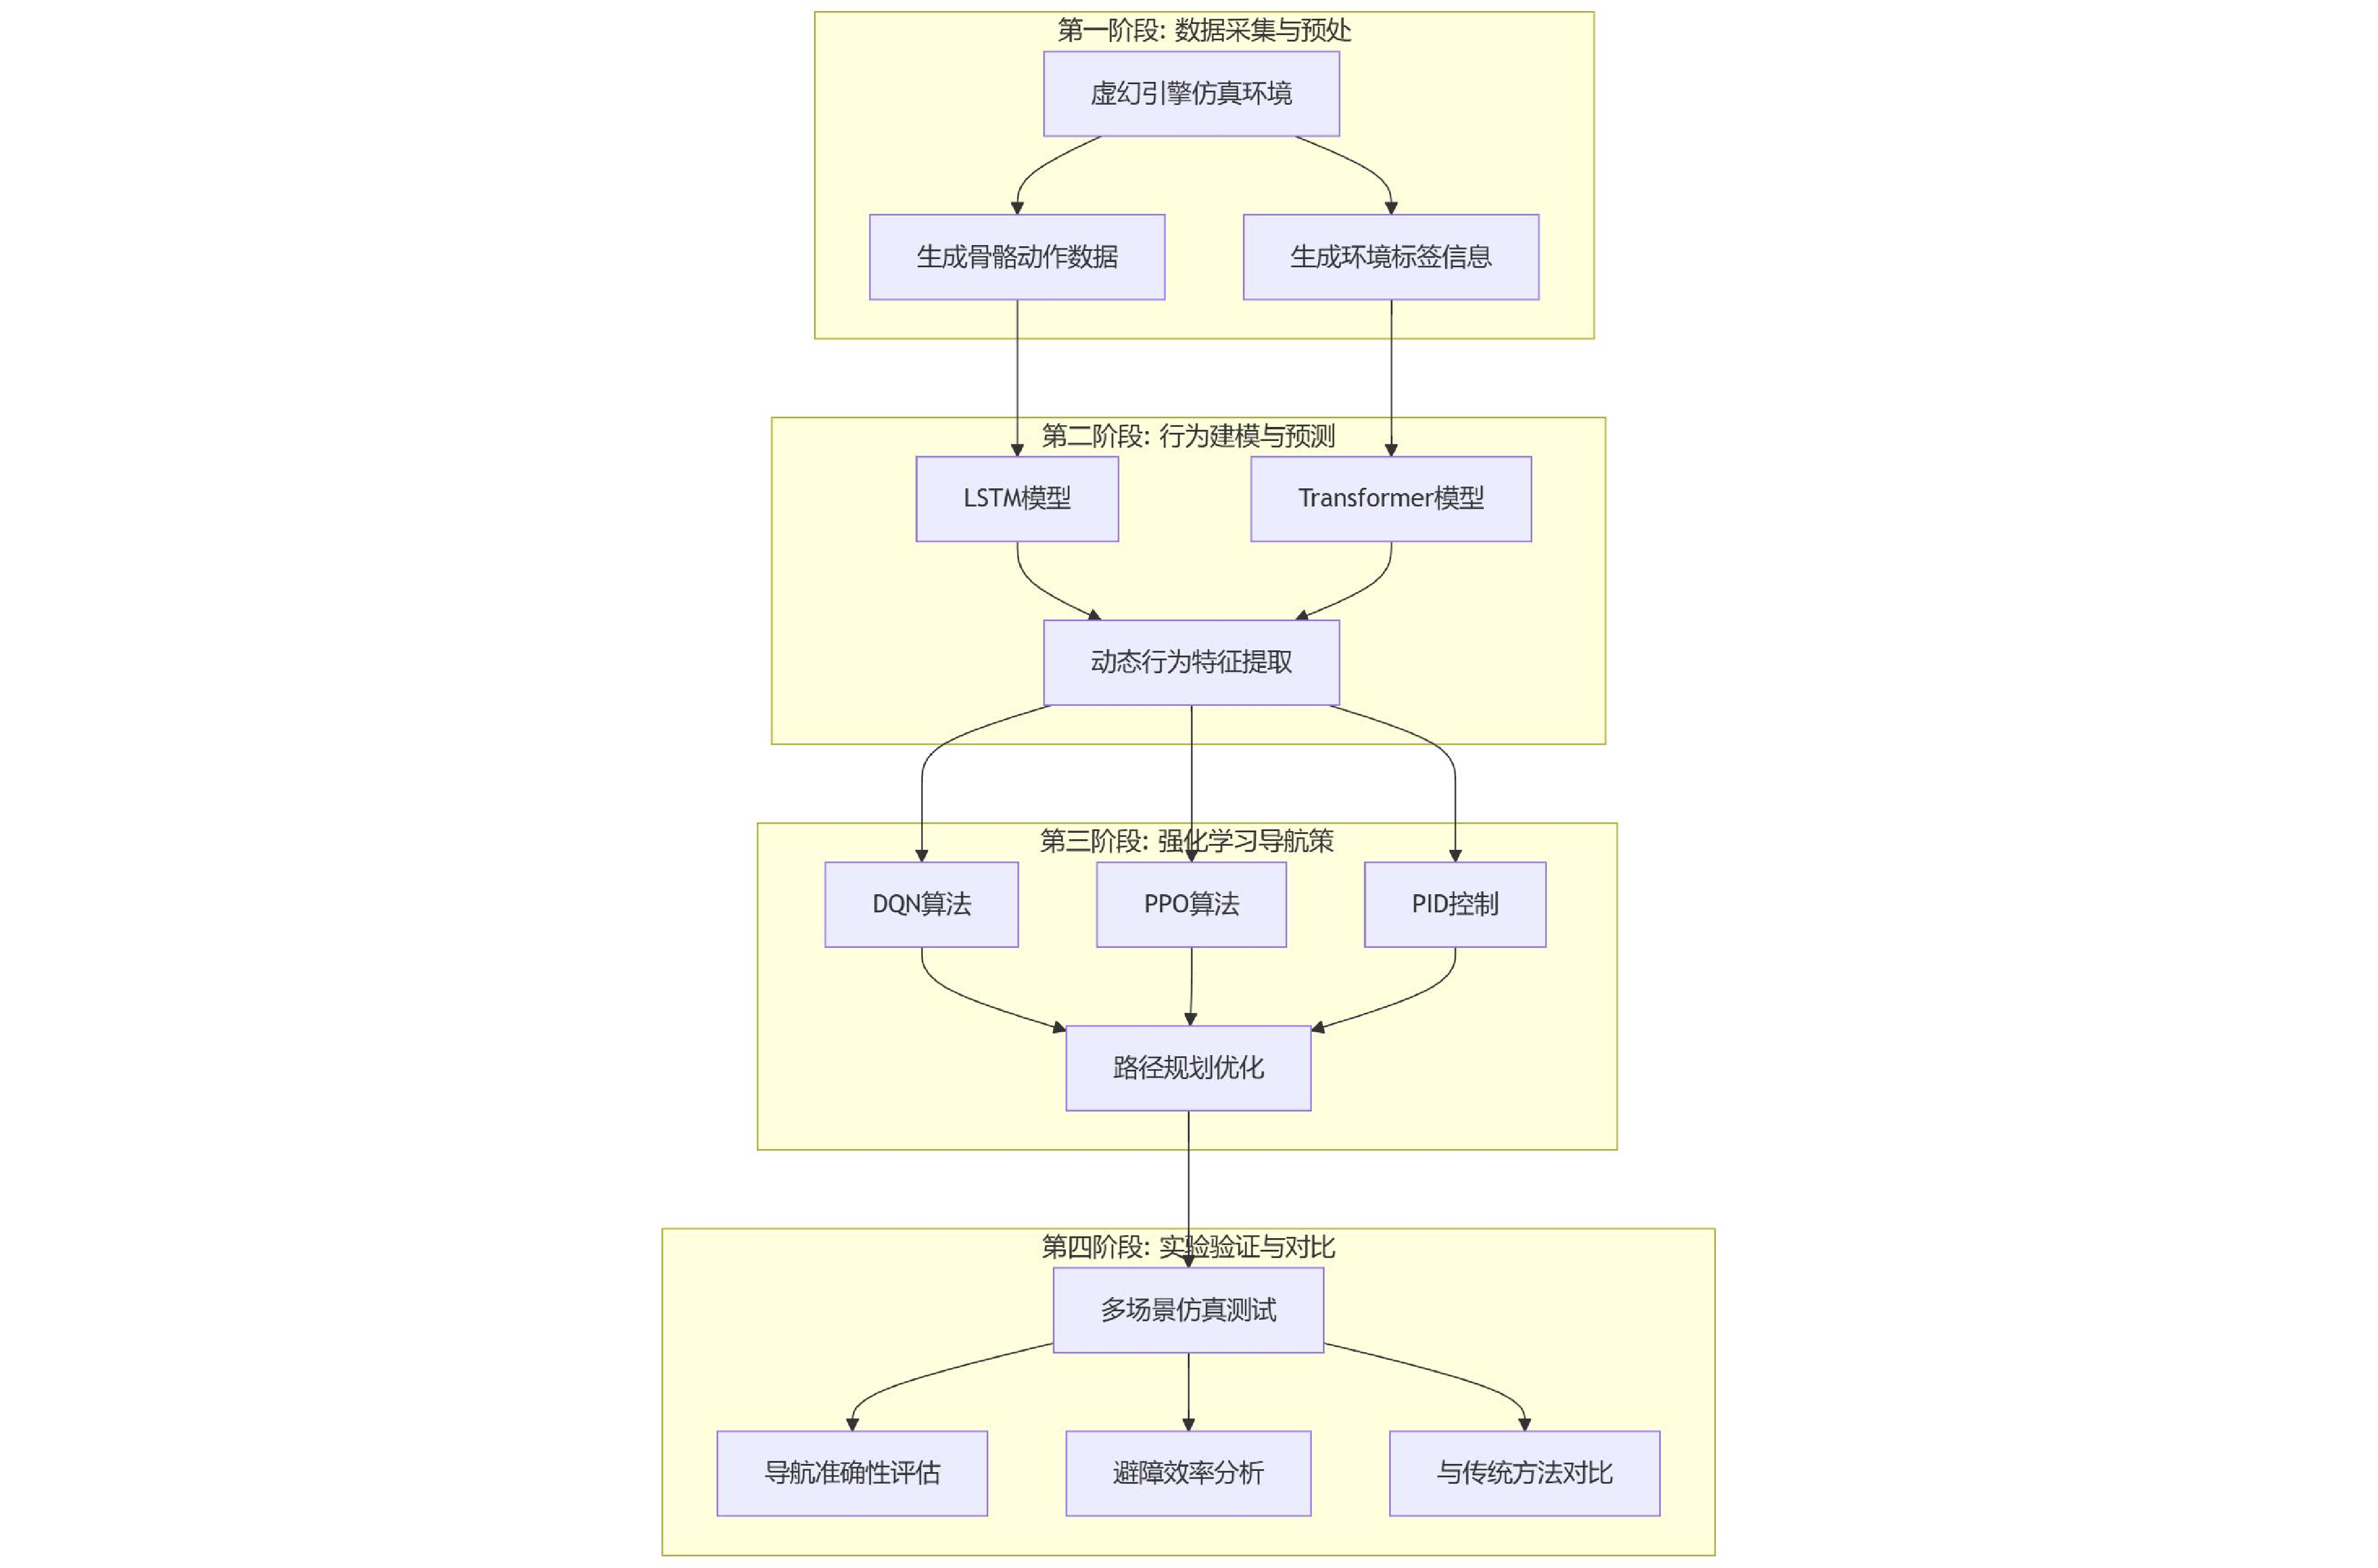
\includegraphics[width=0.8\textwidth]{images/tech_route.pdf}
    \caption{论文技术路线图}
    \label{fig:techroute}
\end{figure}

图\ref{fig:techroute} 展示了本文的整体技术路线,按照“需求分析—平台搭建—算法实现—系统设计—性能评估—未来拓展”的顺序展开,形成一条从理论研究到系统落地的闭环路径。通过虚拟仿真场景设计与Carla平台集成,实现复杂交通场景下的动态障碍物建模与多传感器数据融合;在此基础上实现PID、DQN与PPO等多种强化学习策略控制,并进行对比分析;最终完成行人导航系统的完整功能设计与实验验证,为未来在真实场景中的迁移与多智能体协作提供技术支撑,详细解释如下:

1. \textbf{虚拟仿真环境搭建}:基于虚幻引擎与 Carla 平台构建面向行人导航的高保真虚拟仿真场景,包括虚拟城市环境生成、动态障碍物模拟、多传感器信息建模与数据融合,为强化学习智能体提供训练环境基础。

2. \textbf{强化学习算法实现}:强化学习算法实现部分介绍 PID 控制、DQN 算法与 PPO 策略训练的原理及实现过程,通过对比不同控制策略在复杂环境中的适应性与学习效率为后续导航系统算法选择提供依据。

3. \textbf{行人导航系统设计}:行人导航系统设计围绕行人路径规划与避障问题构建多维奖励函数体系、路径规划模块及避障协同机制,同时建立骨骼控制与行为建模方法并引入动态权重融合策略以提升导航策略的稳定性与效率。

4. \textbf{实验验证与性能评估}:实验验证与性能评估环节通过仿真实验对导航精度、避障成功率、路径效率及实时控制性能进行综合分析,评估不同控制算法在复杂场景下的性能差异及系统整体运行效果。

5. \textbf{未来研究方向}:结合当前成果与系统运行反馈提出未来研究拓展方向,包括多智能体协作机制、传感器系统增强、复杂场景泛化能力提升及算法在硬件部署中的适应性问题。

